\begin{figure}[!htbp]
\centering
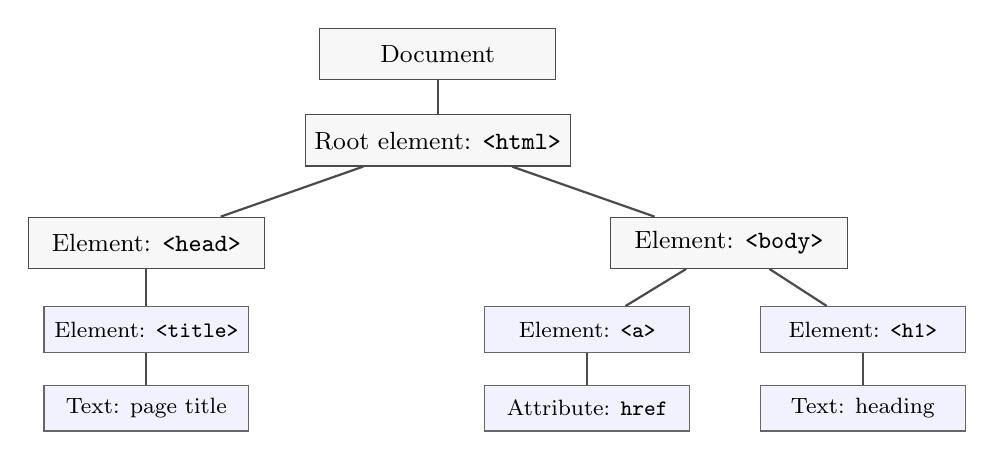
\begin{tikzpicture}[
  domnode/.style={draw=black!70, fill=gray!6, rectangle, minimum width=3.0cm,
                  minimum height=0.65cm, align=center, font=\small},
  leaf/.style={draw=black!60, fill=blue!5, rectangle, minimum width=2.6cm,
               minimum height=0.58cm, align=center, font=\footnotesize},
  domarr/.style={-, thick, black!70}
]
\node[domnode] (doc) at (0,0) {Document};
\node[domnode] (html) at (0,-1.1) {Root element: \texttt{<html>}};
\node[domnode] (head) at (-3.7,-2.4) {Element: \texttt{<head>}};
\node[domnode] (body) at (3.7,-2.4) {Element: \texttt{<body>}};
\node[leaf] (title) at (-3.7,-3.5) {Element: \texttt{<title>}};
\node[leaf] (ttext) at (-3.7,-4.5) {Text: page title};
\node[leaf] (a) at (1.9,-3.5) {Element: \texttt{<a>}};
\node[leaf] (href) at (1.9,-4.5) {Attribute: \texttt{href}};
\node[leaf] (h1) at (5.4,-3.5) {Element: \texttt{<h1>}};
\node[leaf] (htext) at (5.4,-4.5) {Text: heading};

\draw[domarr] (doc) -- (html);
\draw[domarr] (html) -- (head);
\draw[domarr] (html) -- (body);
\draw[domarr] (head) -- (title);
\draw[domarr] (title) -- (ttext);
\draw[domarr] (body) -- (a);
\draw[domarr] (a) -- (href);
\draw[domarr] (body) -- (h1);
\draw[domarr] (h1) -- (htext);
\end{tikzpicture}
\caption{Simplified DOM tree showing how a browser represents an HTML document.}
\label{fig:dom-tree-general}
\end{figure}
